\documentclass[twocolumn]{aastex631}
\usepackage{showyourwork}
\usepackage{amsfonts,amssymb,amsmath}

\begin{document}

\title{Constraining gravitational wave amplitude birefringence with GWTC-3}

\author{Thomas C.K. Ng}
\email{thomas.ng@link.cuhk.edu.hk}
\affiliation{Department of Physics and Institute of Theoretical Physics, The Chinese University of Hong Kong, Shatin, Hong Kong}

\author{Maximiliano Isi}
\email{misi@flatironinstitute.org}
\affiliation{Center for Computational Astrophysics, Flatiron Institute, 162 5th Ave, New York, NY 10010, United States}

\author{Kaze W. K. Wong}
\email{kwong@flatironinstitute.org}
\affiliation{Center for Computational Astrophysics, Flatiron Institute, 162 5th Ave, New York, NY 10010, United States}

\author{Will M. Farr}
\email{wfarr@flatironinstitute.org}
\affiliation{Center for Computational Astrophysics, Flatiron Institute, 162 5th Ave, New York, NY 10010, United States}
\affiliation{Department of Physics and Astronomy, Stony Brook University, Stony Brook NY 11794, United States}

\date{\today}

\begin{abstract}

\end{abstract}

\section{Introduction}

Since Einstein proposed his theory of general relativity (GR), it was tested in a wide range of length scales.
After a century, we know that GR do not agree with quantum theories at some length scale.
To unify both theories, we need to study the possibility of different beyond-GR theories.
Some beyond-GR theories such as Chern-Simons gravity suggested that there is gravitational wave (GW) amplitude birefringence,
while GR predicts there is no birefringence.

\begin{figure}[h!]
    \script{birefringence.py}
    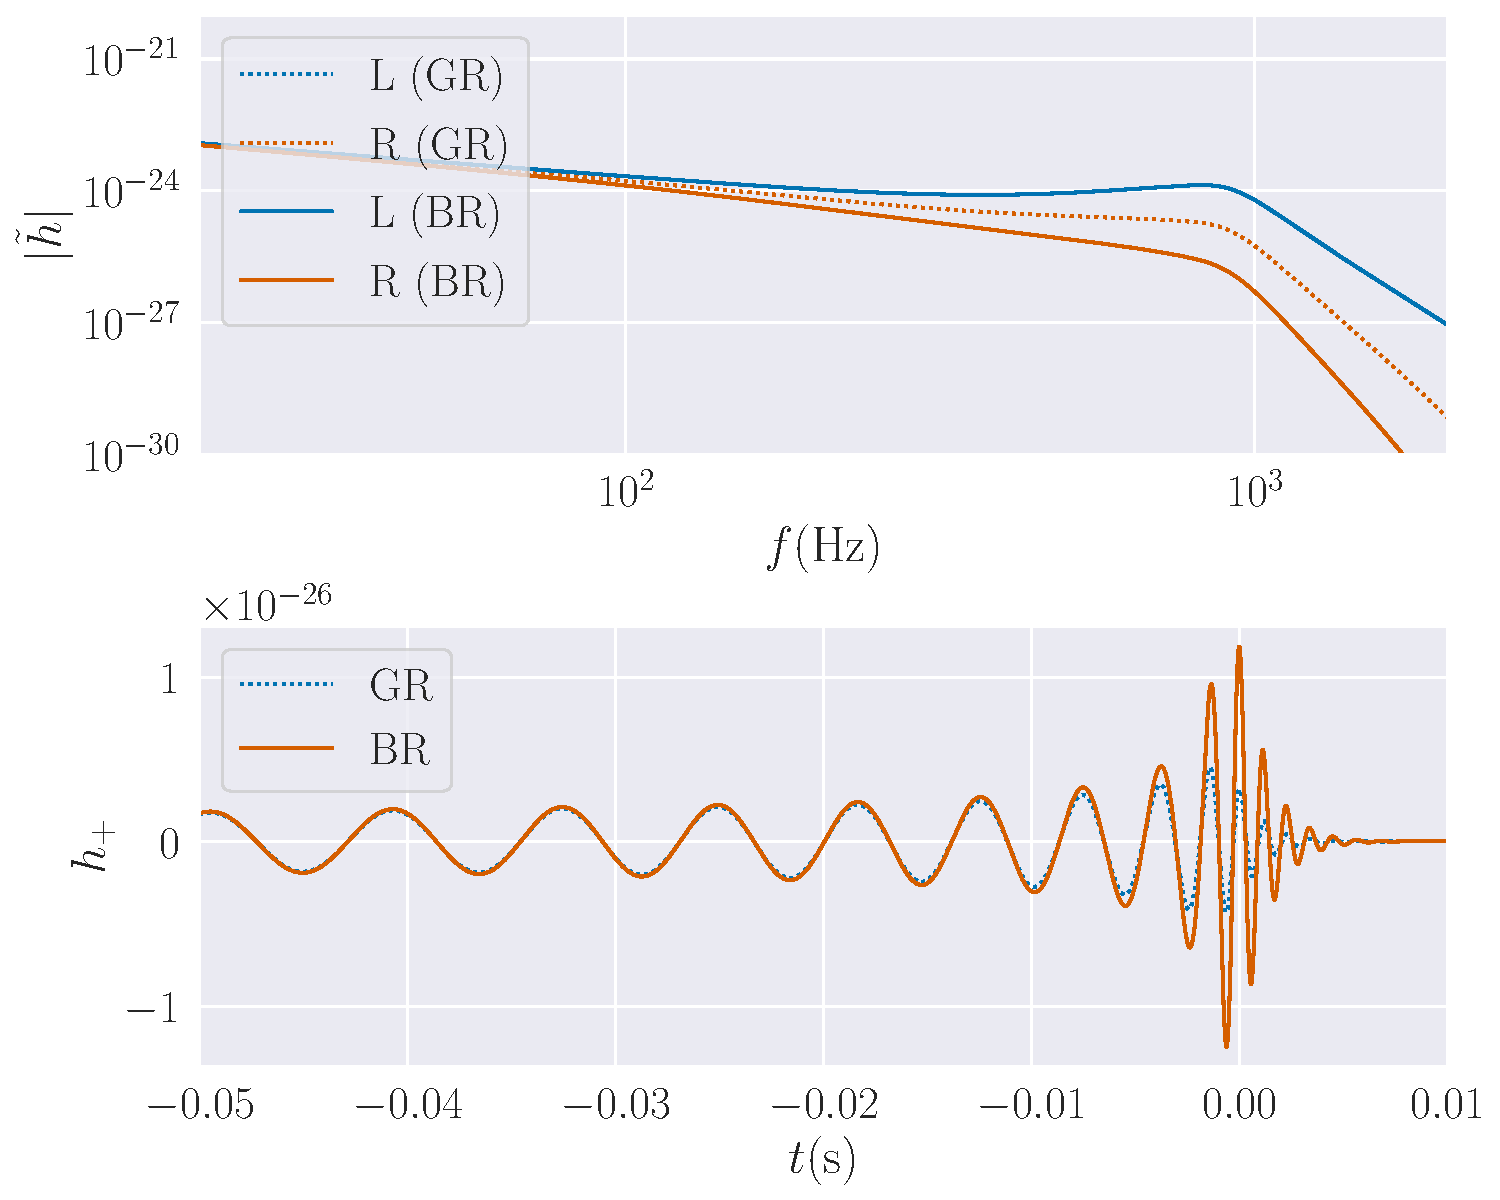
\includegraphics[width=\columnwidth]{figures/birefringence.png}
    \caption{
        The observed amplitudes of two polarisations of an artificial GW signal under different model.
        The top panel shows the case of GR, the amplitudes are unmodified.
        For the middle and bottom panel, they shows the case of birefringence.
        Left-handed polarisation is favored by the birefringence in the middle panel,
        and right-handed polarisation is favored by the birefringence in the bottom panel.
    }
    \label{fig:birefringence}
\end{figure}

GW amplitude birefringence is a property of space which consists of the enhancement of one GW polarisation over the other during the propagation of the wave.
The longer the GW travels, the larger the effect of birefringence.
To illustrate the effect of amplitude birefringence,
the observed amplitudes of two polarisations of an artificial GW signal example are shown in figure \ref{fig:birefringence}.
With birefringence, the amplitude is modified during the propagation,
and the observed amplitudes will be different compare to the amplitudes when they are generated at the binary.

Before we discuss more about GW amplitude birefringence, we need to understand the case of GR.
GW consist of two linear polarizations (i.e. $+$ and $\times$) similar to electromagnetic waves,
which could be transformed into two circular polarizations (i.e. left and right) by $h_{\mathrm{R}, \mathrm{L}} = h_+ \pm i h_\times$.
In GR, the amplitude ratio of the left and right polarisations only depends on the inclination $\iota$ for a nonprecessing binary,
the angle between our line of sight and the orbital angular momentum of the binary.
\begin{equation}
    \left(\frac{h_\mathrm{L}}{h_\mathrm{R}}\right)_\mathrm{GR}=\left(\frac{1-\cos\iota}{1+\cos\iota}\right)^2\,,
\end{equation}where $h_L$ and $h_R$ are the Fourier amplitude of left and right polarizations of the GWs respectively.

For previous studies on the birefringence property such as \citet{Maria_2021}, the amplitude ratio depends on not only $\iota$,
but also the distance to the binary and the strength of the birefringence.
\begin{equation}
    \left(\frac{h_\mathrm{L_{obs}}}{h_\mathrm{R_{obs}}}\right)_\mathrm{Biref}^\mathrm{old}=\frac{e^{d_C\widetilde{\kappa}}\left(1-\cos\iota\right)^2}{e^{-d_C\widetilde{\kappa}}\left(1+\cos\iota\right)^2}\,,
\end{equation}where $d_C$ is the comoving distance to the binary, $\widetilde{\kappa}$ is the opacity parameter that represent
the strength of the birefringence with units of $L^{-1}$, and $h_\mathrm{L_{obs}}$ and $h_\mathrm{R_{obs}}$ are
the observed Fourier amplitude of left and right polarizations of the GW respectively. Note that GR is recovered if $\kappa$ is $0$.
This is a zeroth-order approximation of the birefringence model in Chern-Simons gravity, which assume there is no frequency dependence.
This would create a degeneracy between kappa and iota, as they can affect the amplitude ratio in the same way.

In this paper, we considered the frequency dependence of the birefringence as well.
Thus, the amplitude ratio of the left and right polarisations will be as follow.
\begin{equation}
    \left(\frac{h_\mathrm{L_{obs}}}{h_\mathrm{R_{obs}}}\right)_\mathrm{Biref}^\mathrm{new}=\frac{\exp\left({\kappa\frac{d_C}{1\mathrm{ Gpc}}\frac{f}{100\mathrm{ Hz}}}\right)\left(1-\cos\iota\right)^2}{\exp\left({-\kappa\frac{d_C}{1\mathrm{Gpc}}\frac{f}{100\mathrm{Hz}}}\right)\left(1+\cos\iota\right)^2}\,,
\end{equation}where $f$ is the frequency of the GWs and $\kappa$ is the dimensionless opacity parameter that represent the strength of the birefringence.
This frequency dependence provides stronger enhancement or suppression from the birefringence to high frequency components of the GW, and visa versa.
Also, the frequency dependence can break the degeneracy between kappa and iota,
as this would make the effect of the birefringence affect the amplitude ratio differently compared to iota.

\section{Method}

To constrain $\kappa$, we perform parameter estimation (PE) with data from the third LIGO-Virgo catalog \citep{GWTC-2.1, GWTC-3}, GWTC-3, using Bilby,
a Bayesian toolkit for GW data analysis which is able to calculate posteriors of GW parameters based on interferometer data
and priors for the parameters in question. \citep{Bilby}

We assume GWs are generated at the binary as GR described. As the GWs propagate through space,
the effect of the birefringence will be built up as the distance increases.
To implement the amplitude birefringence on Bilby, waveforms are modified according to the following equation:
\begin{equation}
    h_\mathrm{L,R}^{\mathrm{Biref}}=
    h_\mathrm{L,R}^{\mathrm{GR}}\times
    \exp\left(\pm\kappa\frac{d_C}{1\mathrm{ Gpc}}\frac{f}{100\mathrm{ Hz}}\right)\,.
\end{equation}
This modification allows Bilby to perform estimations on $\kappa$, as the waveforms will depends on $\kappa$ as well.

After modifying Bilby, we set the prior on $\kappa$ to be a $\delta$ function at $0$, which is the same as using GR,
to test if the PEs could recover the PE done by LIGO in \citet{GWTC-2.1, GWTC-3}. These control tests result can be found in the data release.
We then set the prior on $\kappa$ to a uniform function between $-1$ and $1$, and perform PEs on the modified waveforms.
In both case, we use the same configuration as in \citep{GWTC-2.1, GWTC-3} for each individual events.

\section{Results}

\subsection{Result for GW150914}

\begin{figure}[h!]
    \script{GW150914_corner.py}
    \includegraphics[width=\columnwidth]{figures/GW150914_corner.png}
    \caption{
        The posterior of $\kappa$, luminosity distance $d_L$ and $\cos{\iota}$ for GW150914.
    The three sets of plots are the PEs done by LIGO with GR \citep{GWTC-2.1, GWTC-3},
    the PE done by us with the frequency independent birefringence and the frequency dependent birefringence respectively.
    Note that there is no posterior of $\kappa$ for the PE from LIGO, as the LIGO PE is based on GR,
    which does not suggest GW amplitude birefringence.
    }
    \label{fig:GW150914_corner}
\end{figure}

Consider GW150914, the first detected GW by LIGO. In figure \ref{fig:GW150914_corner}, the posteriors of the parameters of the GW150914 is shown.
With the frequency independent birefringence model, the posteriors for $\cos\iota$ look different from the posteriors assuming GR.
This is because, for a nonprecessing system, there is a degeneracy between $\kappa$ and $\iota$ if the frequency dependence is not included.
To reconstruct the amplitude ratio from the interferometer data, an $\iota$ representing a more face-off inspiral can pair with a positive $\kappa$,
or an $\iota$ representing a more face-on inspiral with a negative $\kappa$.
As a result,many pairs of $\iota$ and $\kappa$ can be plausible with the frequency independence.

On the other hand, with the frequency-dependent birefringence model, the posterior looks similar to the GR posterior.
This is because the degeneracy was broken by the frequency dependence, as the effect of the birefringence will be different from the one of changing $\iota$.
In this case, the posteriors can recover the GR distributions for the binary parameters,
and the most probable value of $\kappa$ is close to $0$, which means the birefringence is weak or absent, and GR can be recovered.

\subsection{Result on GWTC-3}

We then perform PE on $71$ binary black hole merger events in GWTC-3 to further constrain $\kappa$.
The posteriors for $\kappa$ of the events are shown in figure \textbf{[X]}, which shows $\kappa$ tend to be $0$.
The combined posterior for $\kappa$ was calculated and shown in figure \textbf{[X]}, which allows us to constrain $\kappa$ within \textbf{[the number we get]}.

\section{Discussion}

\subsection{Limitation}



\subsection{Future Study}



\section{Acknowledgements}



\bibliography{bib}

\section{Points}

\begin{enumerate}
    \item Introduction
    \begin{enumerate}
        \item Motivation
        \begin{enumerate}
            \item GR broke down at some scale, find a new theory
            \item CS: beyond-GR theory
            \item test CS property (GW amplitude birefringence)
        \end{enumerate}
        \item Amplitude Birefringence
        \begin{enumerate}
            \item GW amplitude birefringence is a property of space
            \item birefringence: enhance one and suppress another
            \item figure to illustrate the effect of birefringence
        \end{enumerate}
        \item Amplitude Ratio
        \begin{enumerate}
            \item GR: amplitude ratio depends on $\iota$ only
            \item nonGR: also depends on $\kappa$, $d_C$ and $f$
        \end{enumerate}
    \end{enumerate}
    \item Method
    \begin{enumerate}
        \item Parameter Estimation
        \begin{enumerate}
            \item PE on GWTC-3 to constrain $\kappa$
            \item Assume GW are generated as GR described
            \item birefringence is considered during the propagation
            \item waveform modification
            \item GR control test
            \item same configuration as LIGO
        \end{enumerate}
    \end{enumerate}
    \item Results
    \begin{enumerate}
        \item GW150914
        \begin{enumerate}
            \item figure with frequency-dependent and frequency-independent
            \item posterior from $\cos\iota$ looks different
            \item frequency-dependent: degeneracy between $\iota$ and $\kappa$
            \item frequency-independent: degeneracy broken and $\kappa$ near $0$
        \end{enumerate}
        \item GWTC-3
        \begin{enumerate}
            \item figure of $\kappa$ of all events
            \item constraint on $\kappa$
            \item improvement of constraint on $\kappa$ compare to previous studies
        \end{enumerate}
    \end{enumerate}
    \item Discussion
    \begin{enumerate}
        \item Limitation
        \begin{enumerate}
            \item orientation of detector (polarisations)
            \item sensitivity of detector
        \end{enumerate}
        \item Future Study
        \begin{enumerate}
            \item More events from detector
            \item Higher order terms
        \end{enumerate}
    \end{enumerate}
\end{enumerate}

\end{document}
